\documentclass{article}
\usepackage{tikz}
\usepackage{graphicx}
\graphicspath{ {./img/} }

\author{Kent Odde, Stian Onarheim, Tarald Vestbøstad}
\title{Title}

\begin{document}

\pagestyle{empty}

 \begin{tikzpicture}[remember picture,overlay]
    \node[anchor=north west,yshift=-15pt,xshift=20pt]%
        at (current page.north west)
        {
\includegraphics[height=8em]{img/USN_logotype.png}};

\end{tikzpicture}


%\vspace{2.5cm}

{\LARGE test}\hspace{2cm}

\begin{tikzpicture}[overlay]
    \node[anchor=north, inner sep=0] at (4,-2)
        {
\includegraphics[width=\textwidth]{img/frontpage-block.png}};
\end{tikzpicture}

\begin{tikzpicture}[overlay]
    \node[anchor=north, inner sep=0] at (-3,-0) {\large Hello};
        
\end{tikzpicture}

\maketitle

\section{Maybe useful text}

Thursday 20. August 2020, the group gathered and had a meeting with Steven Bos. We discussed our project idea and the potential use of the Microsoft HoloLens 2. It was in the group's best interest to put our resources into the microcontroller rather than the goggles, dismissing any development with the HoloLens.

\vspace{5mm}
On September 10. the group met to plan the project. After deciding on the initial design, we drew a sketch and wrote a short description. This was sent to our professor, along with a list of required parts as well as the associated budget. The initial design can be seen in section XX.

\section{Maybe useful pictures}

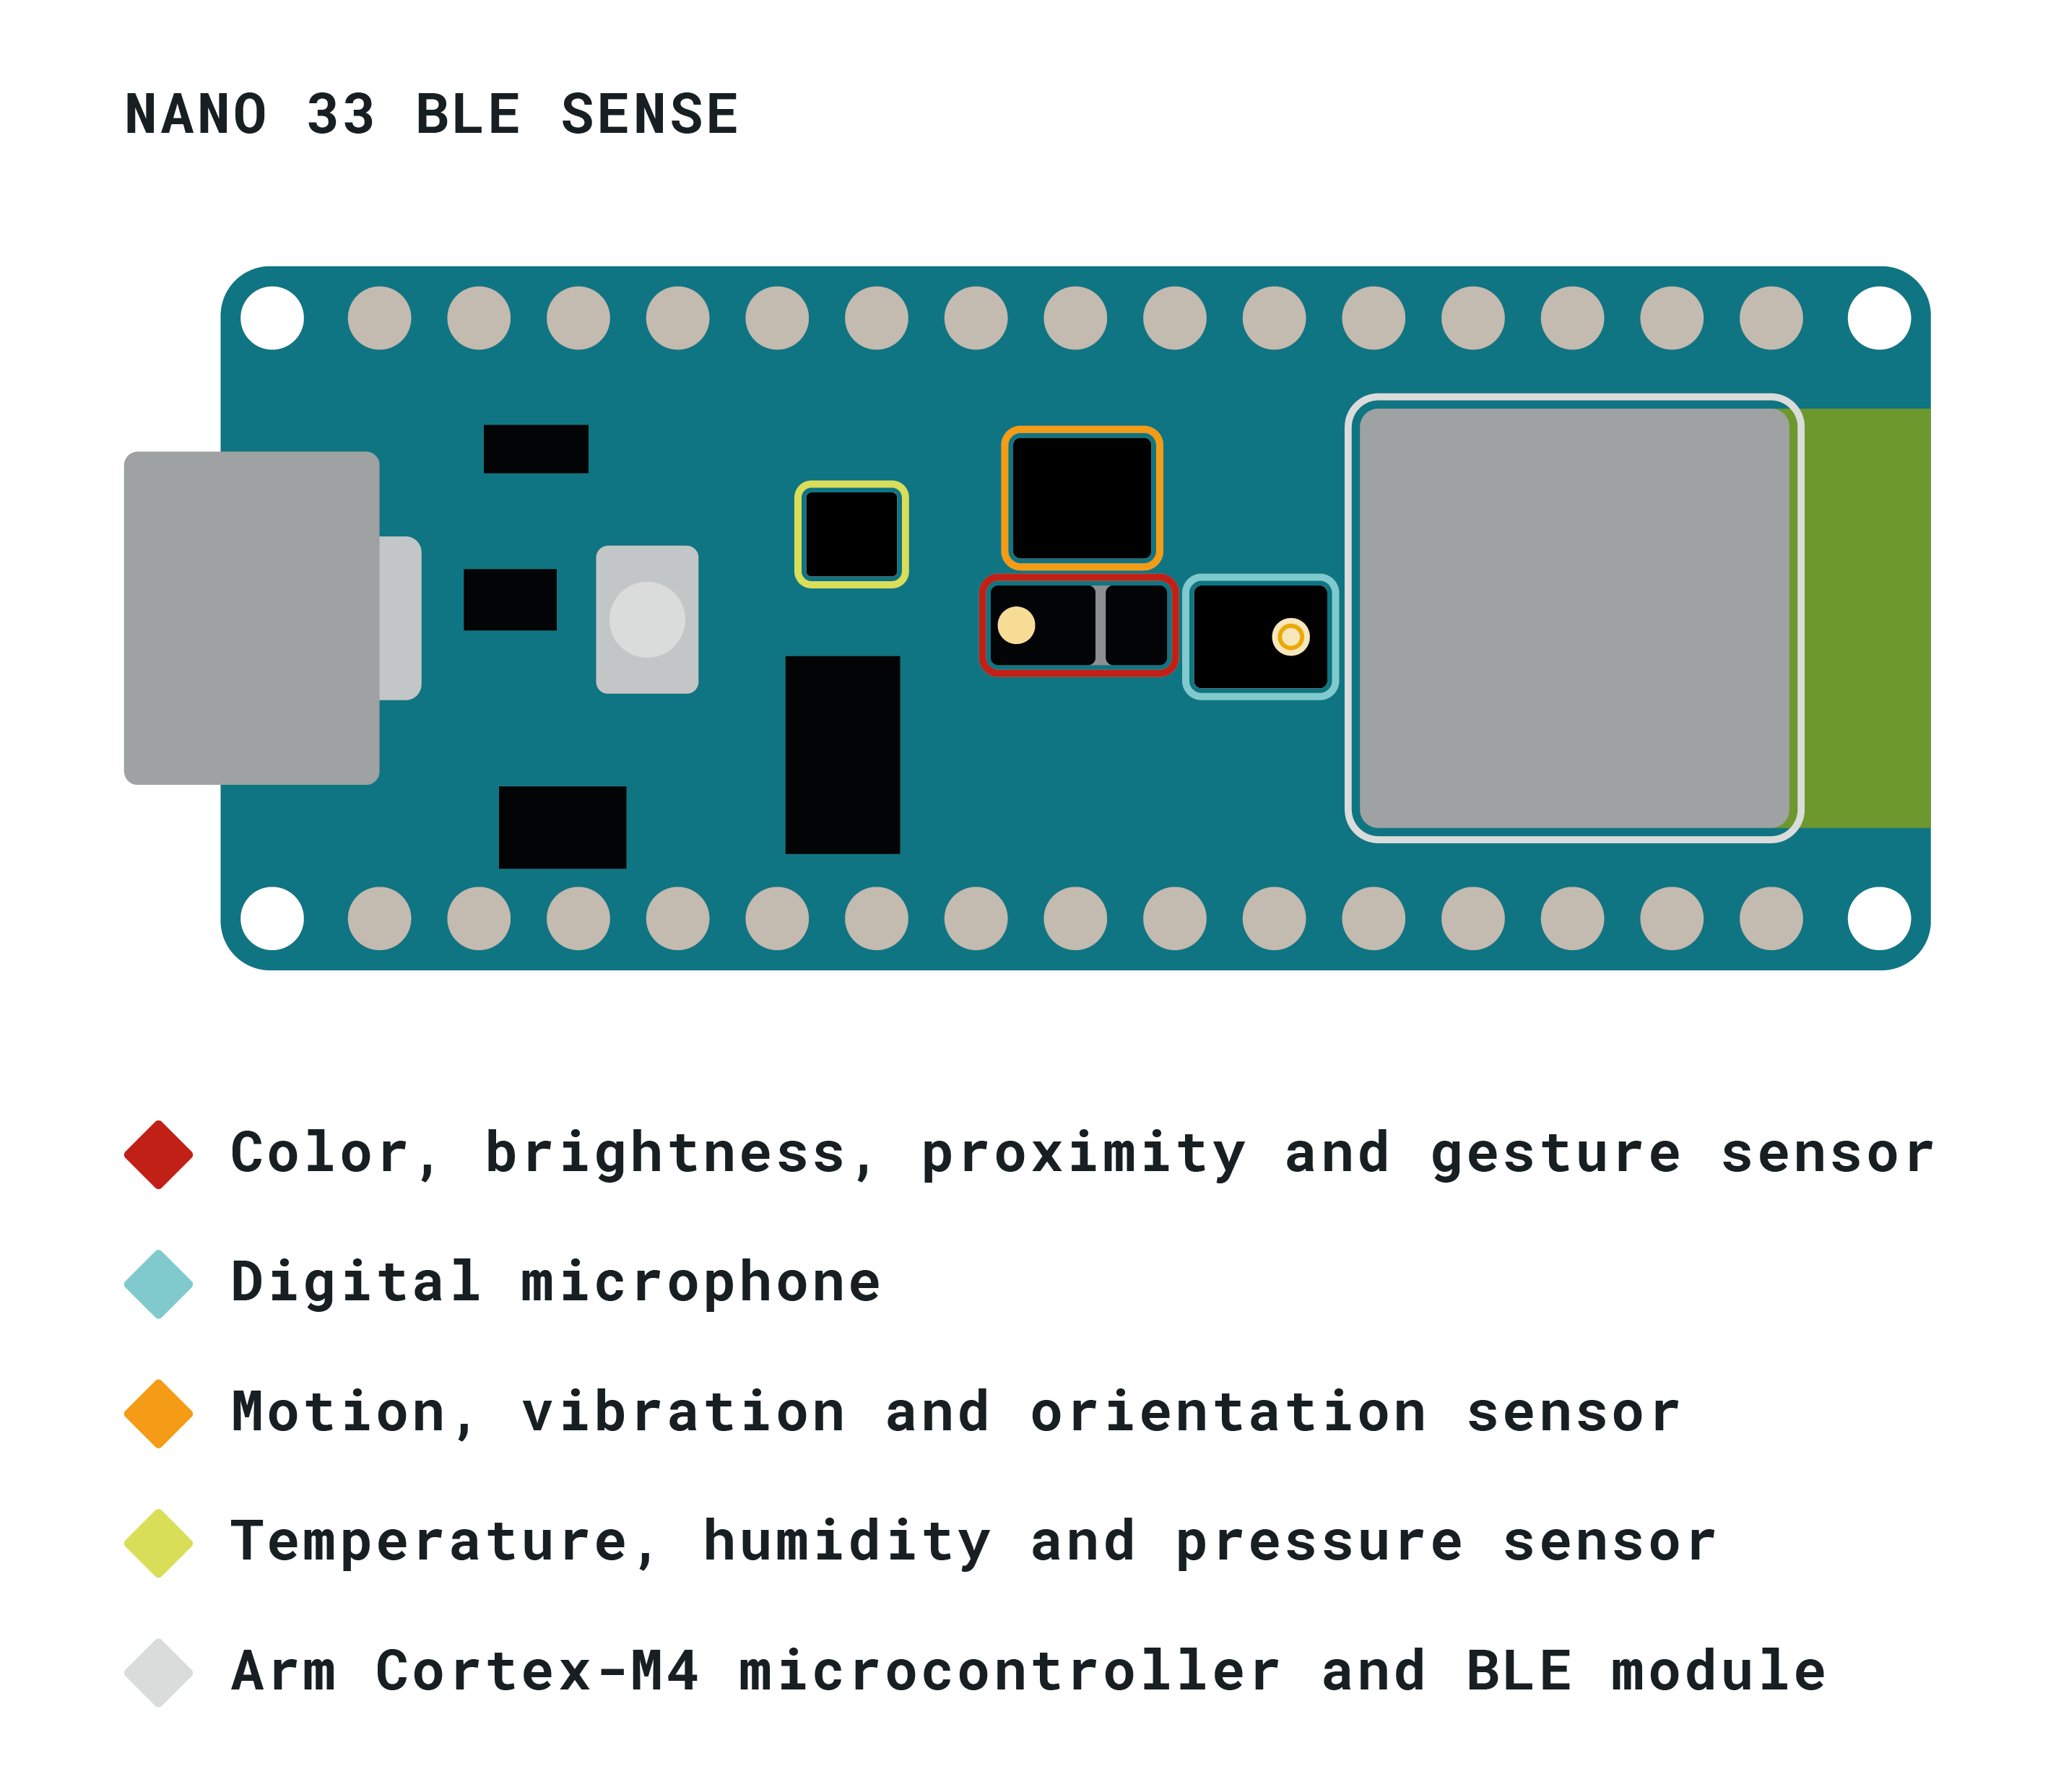
\includegraphics[width=\linewidth]{img/NANO-33-BLE-Sense_sensor-indentification.png}

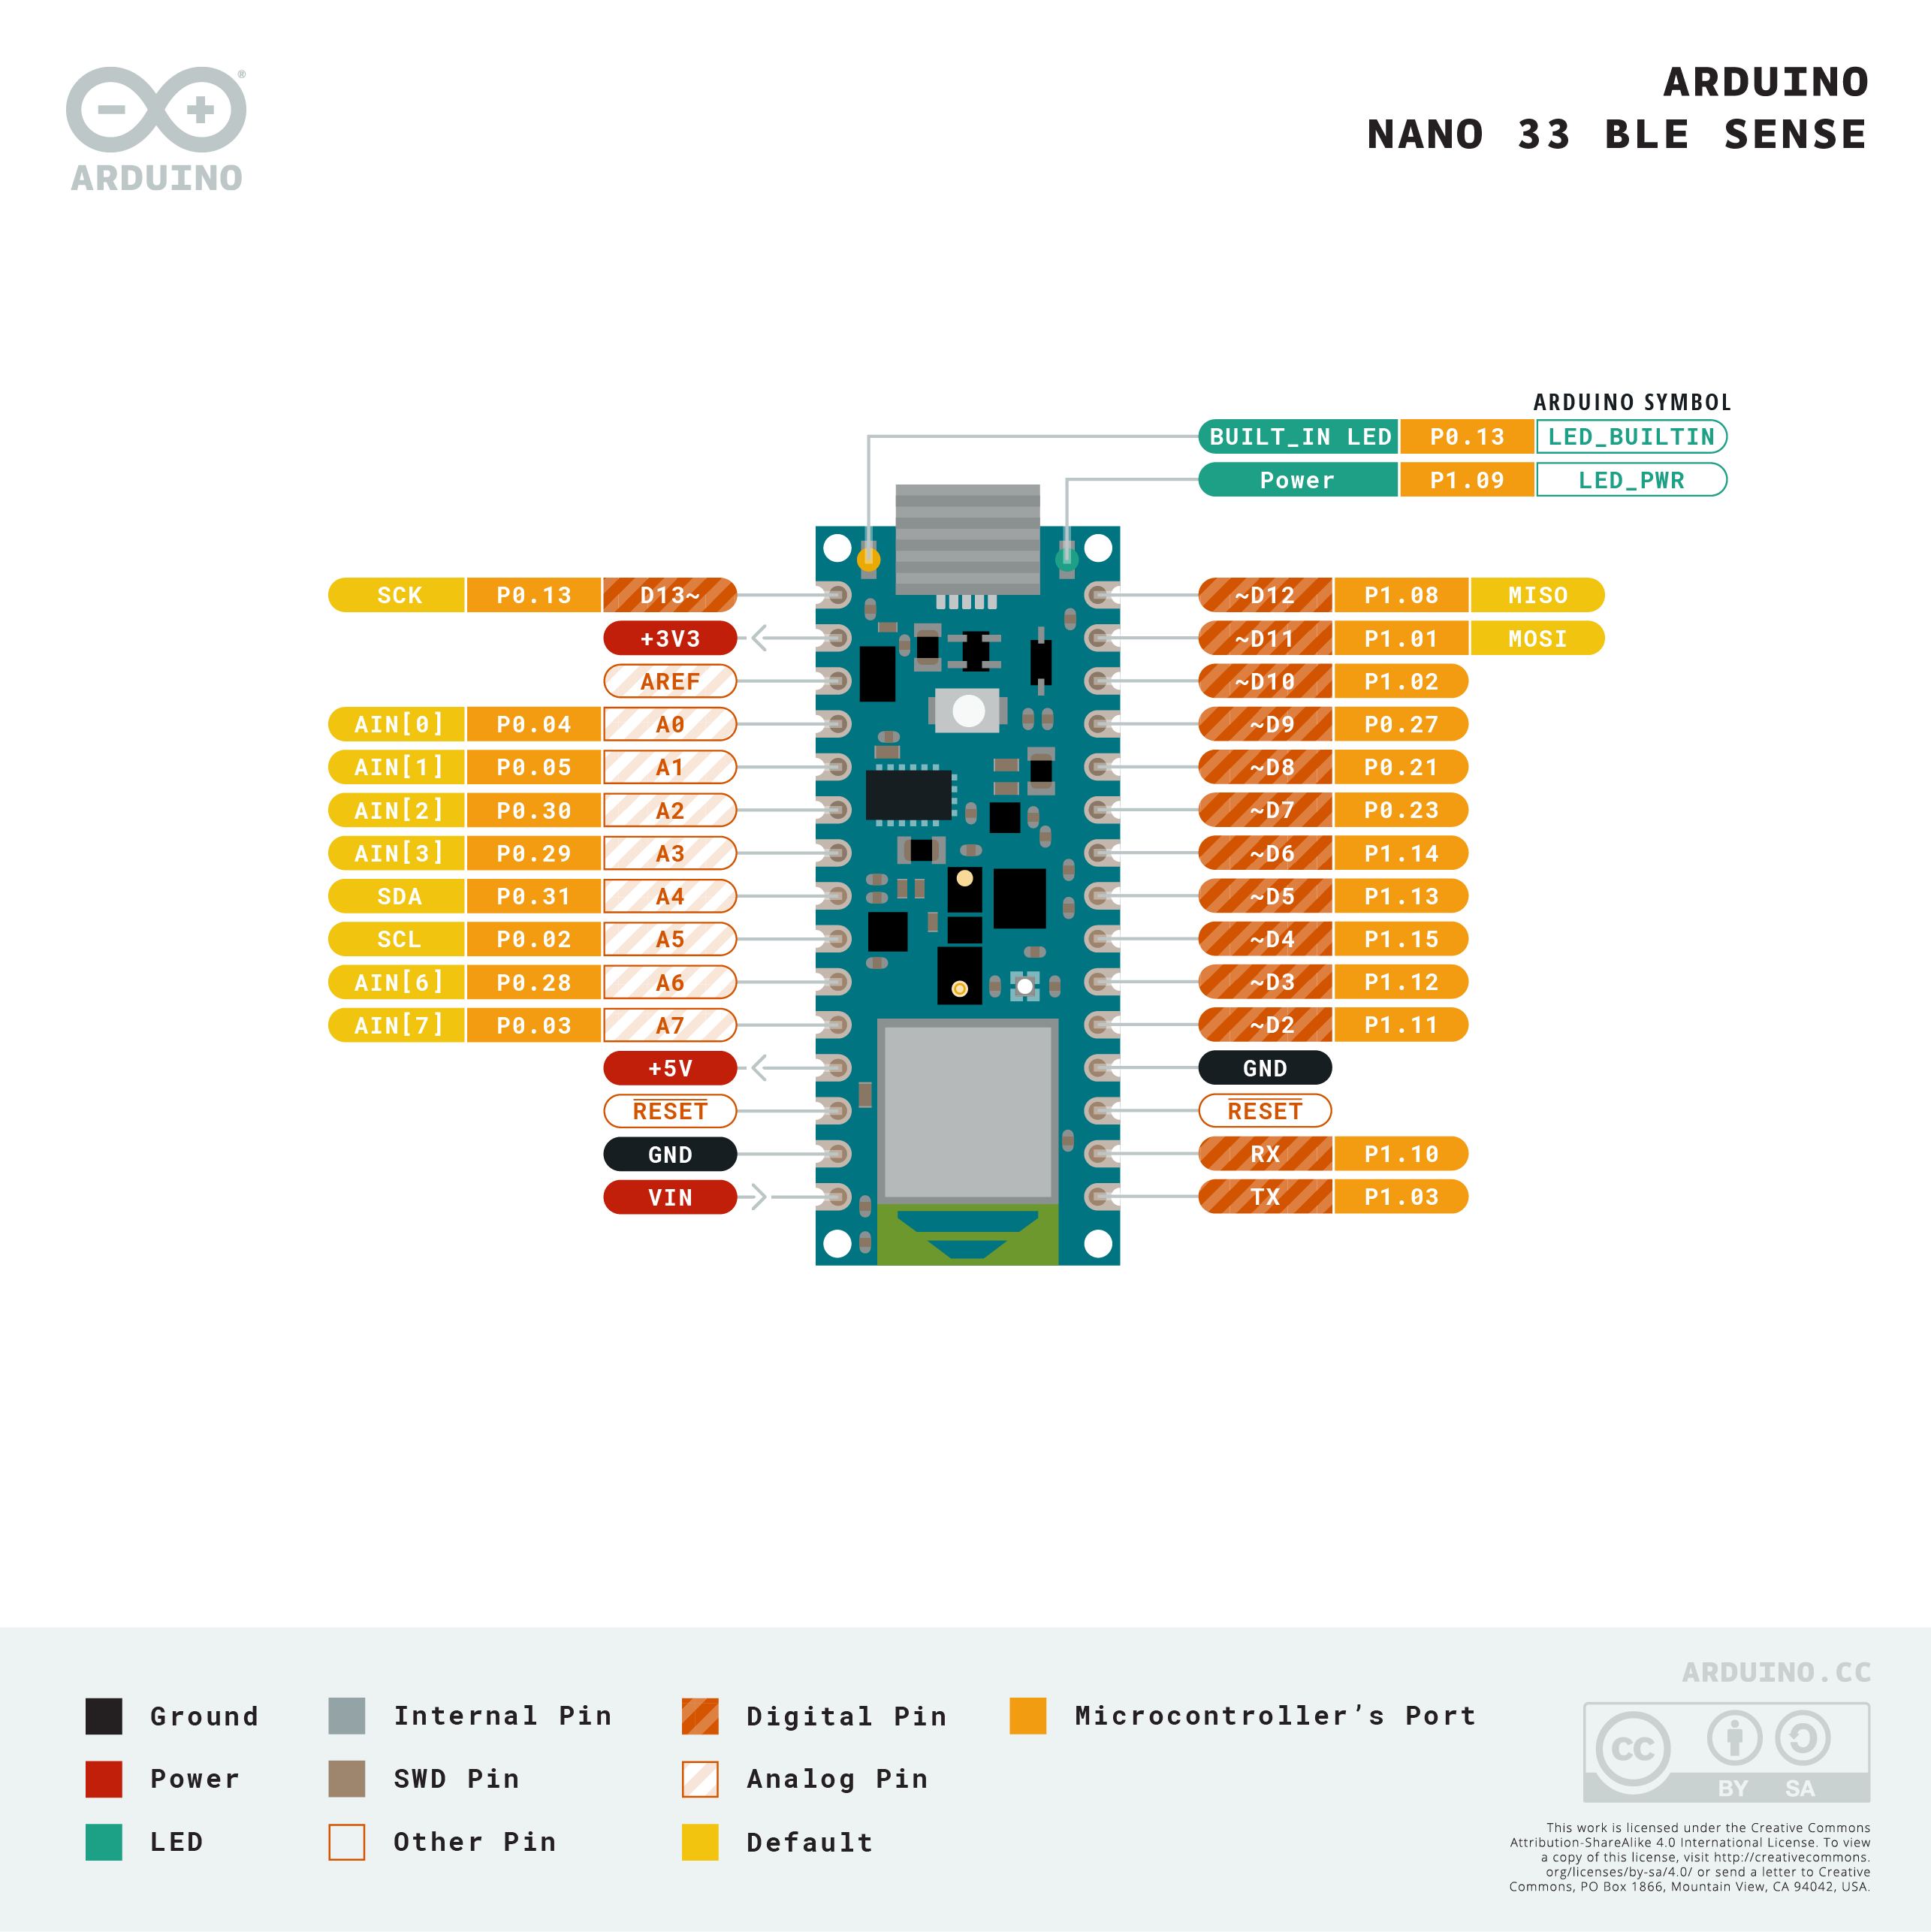
\includegraphics[width=\linewidth]{img/Pinout-NANOsense_latest.png}

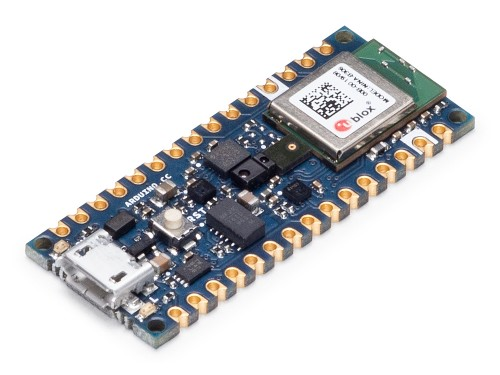
\includegraphics[width=\linewidth]{img/abx00031_iso_1.jpg}

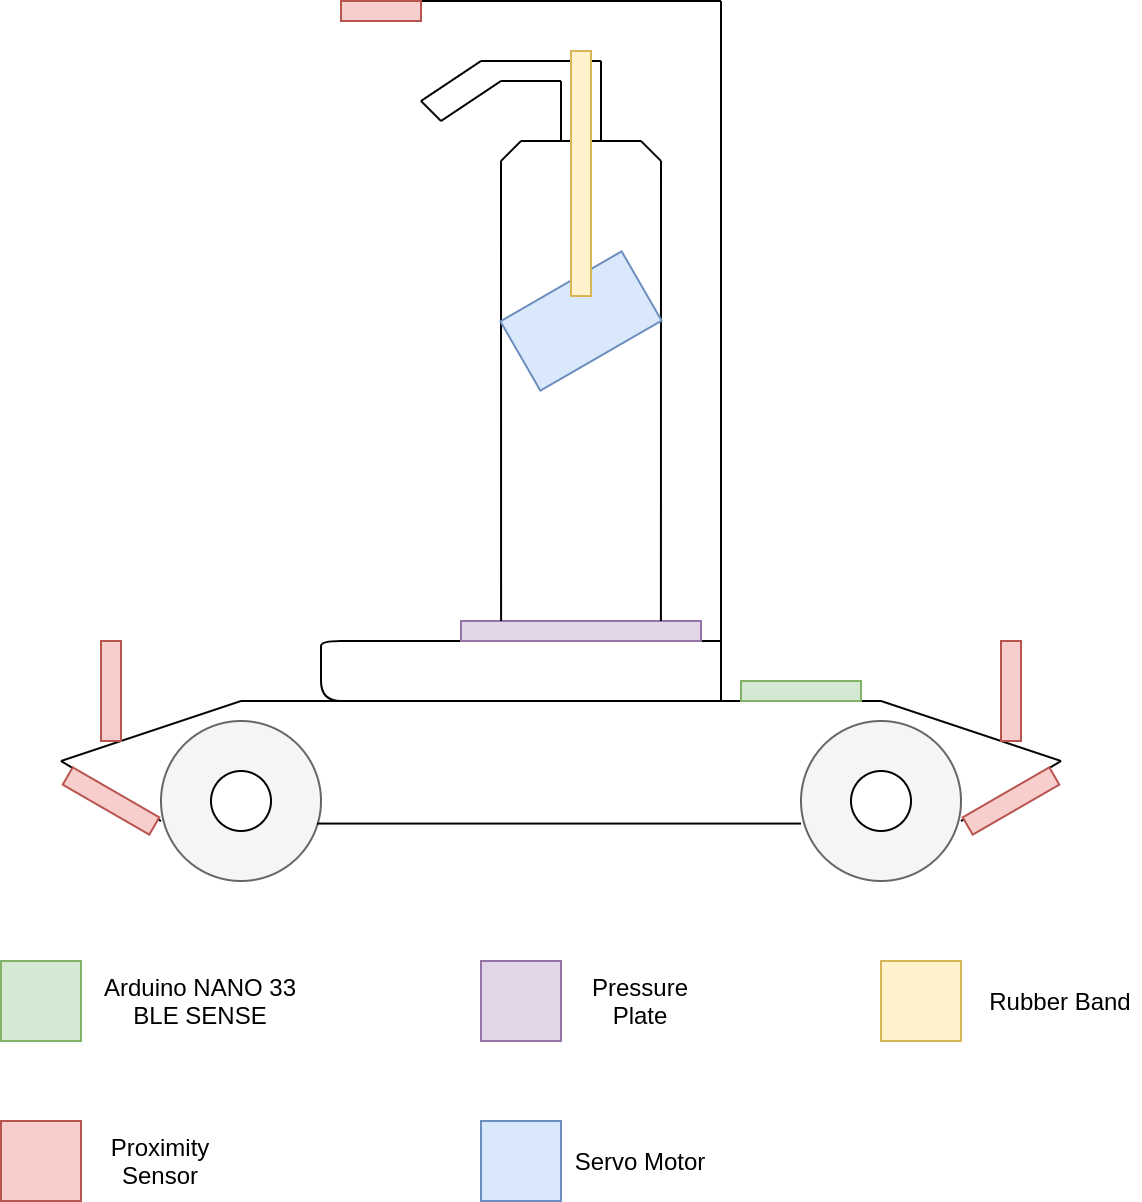
\includegraphics[width=\linewidth]{img/prototype-drawing.png}

\section{Maybe sources}

https://store.arduino.cc/arduino-nano-33-ble-sense\\
https://www.microsoft.com/en-us/hololens/buy


\end{document}

padding oracle attacks.